\section{Results}
An example of a calculated modulation signal $m(t,f)$ caused by fluctuations of the refractive-index in a Gaussian field is shown in figure \ref{fig:modulation_signal}.
The figure shows the log-amplitude and phase fluctuations as function of time for a specific frequency.
% For this example the mean squared refractive-index is $\mu = 3 \cdot 10^{-6}$, the outer length scale $L = 15 $ m, speed of sound $c=343$ m/s, and the distance $r$ 2000 meters. 
% The sample frequency is 10000 Hz and duration of the fragment is 10 seconds.

\Figure{fig:modulation_signal}{Amplitude and phase fluctuations as function of time for 200 Hz. The parameters $\langle \mu^2 \rangle = 3 \cdot 10^{-6}$, $L = 15 $ m, $c=343$ m/s, $r=2000$ m, were used.}
       {60}{ \put(3,3)  {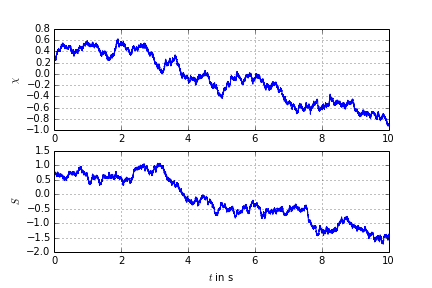
\includegraphics[width=75mm]{../figures/modulation_signal}}}

To check whether the resulting variance of the log-amplitude and phase fluctuations of such a modulation signal are as they should be, a comparison is made with equation \ref{eq:model_daigle}.
The extraction and analysis of the mean square amplitude and phase fluctuations follows the method of Daigle et al.

The mean square log-amplitude fluctuation was calculated as
\begin{equation}
 \langle \chi^2 \rangle = \frac{1}{N} \sum_{n=1}^N \chi_n^2
\end{equation}
where
\begin{equation}
 \chi_n = \ln{\left(A_n/A_m\right)}
\end{equation}
and $A_m$ is the average amplitude over $N$ samples in time
\begin{equation}
 A_m = \frac{1}{N} \sum_{n=1}^N A_n
\end{equation}
where $n$ is the sample at time $t$. Similarly, the mean square of the phase fluctuations is calculated as
\begin{equation}
 \langle S^2 \rangle = \frac{1}{N} \sum_{n=1}^N \left( \phi_n - \phi_m \right)^2
\end{equation}
with
\begin{equation}
 \phi_m = \frac{1}{N} \sum_{n=1}^N \phi_n
\end{equation}


Figure \ref{fig:function_of_frequency} shows the log-amplitude and phase variances as function of frequency. The frequency-dependency is maintained although the variance is slightly lower than expected.

\Figure{fig:function_of_frequency}{Log-amplitude and phase variances as function of frequency. The parameters $\langle \mu^2 \rangle = 3\cdot 10^{-6}$, $L=15$ m, $c=343$ m/s, $r=2000$ m, were used.}
       {60}{ \put(3,3)  {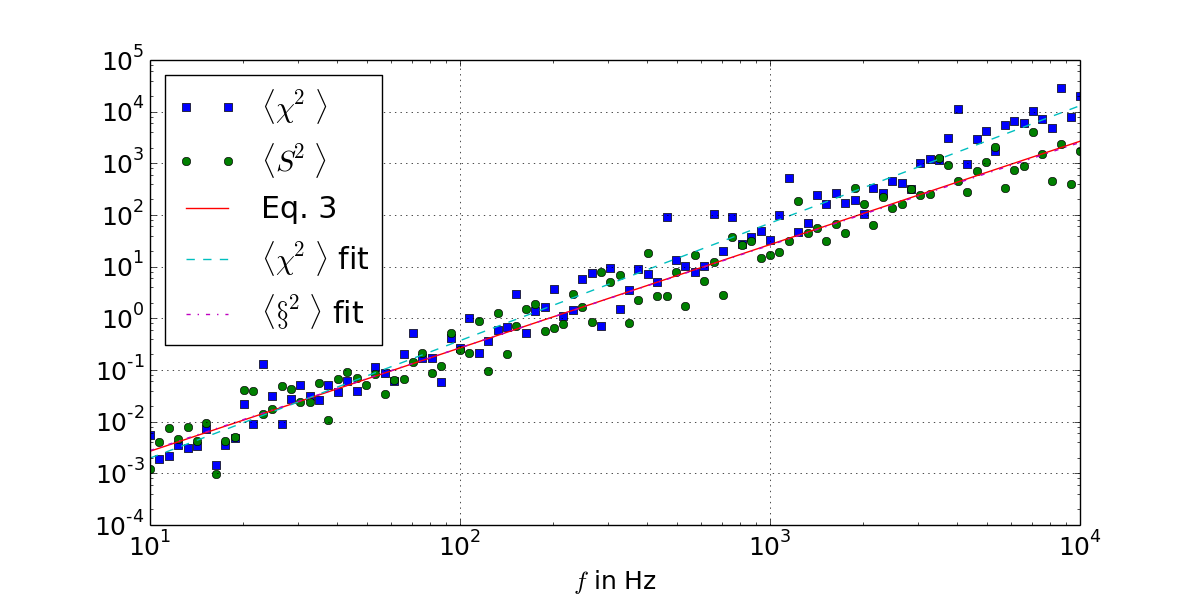
\includegraphics[width=75mm]{../figures/function_of_frequency}}}
       
The same applies to the distance-dependency. Figure \ref{fig:function_of_distance} shows the log-amplitude and phase variances as function of distance. The variance of the fluctuations is also slightly lower than expected.
       
\Figure{fig:function_of_distance}{Log-amplitude and phase variances as function of distance. The parameters $\langle \mu^2 \rangle = 3\cdot 10^{-6}$, $L=15$ m, $c=343$ m/s, $f=200$ Hz, were used.}
       {60}{ \put(3,3)  {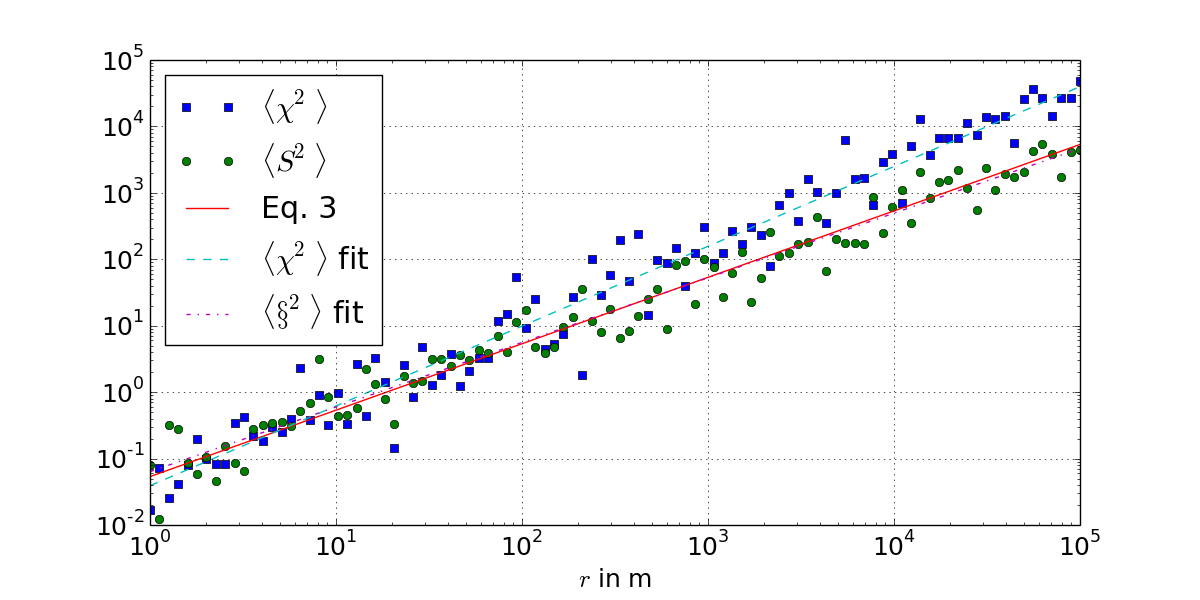
\includegraphics[width=75mm]{../figures/function_of_distance}}}
       
While the simple theory predicts that the mean square log-amplitude and phase fluctuations are equal, Daigle et. al. \cite{Daigle1983} showed through measurements that the log-amplitude fluctuations don't obey the simple theory but are in fact smaller than predicted.
Figure \ref{fig:function_of_distance_with_saturation} shows again the mean square fluctuations as function of distance, but this time taking into account log-amplitude saturation.

\Figure{fig:function_of_distance_with_saturation}{Log-amplitude and phase variances as function of distance taking into account the log-amplitude saturation. 
The same parameters as in \ref{fig:function_of_distance} were used. The distance to saturation $r_s$, calculated using equation \ref{eq:saturation_distance}, was 827 m.}
       {60}{ \put(3,3)  {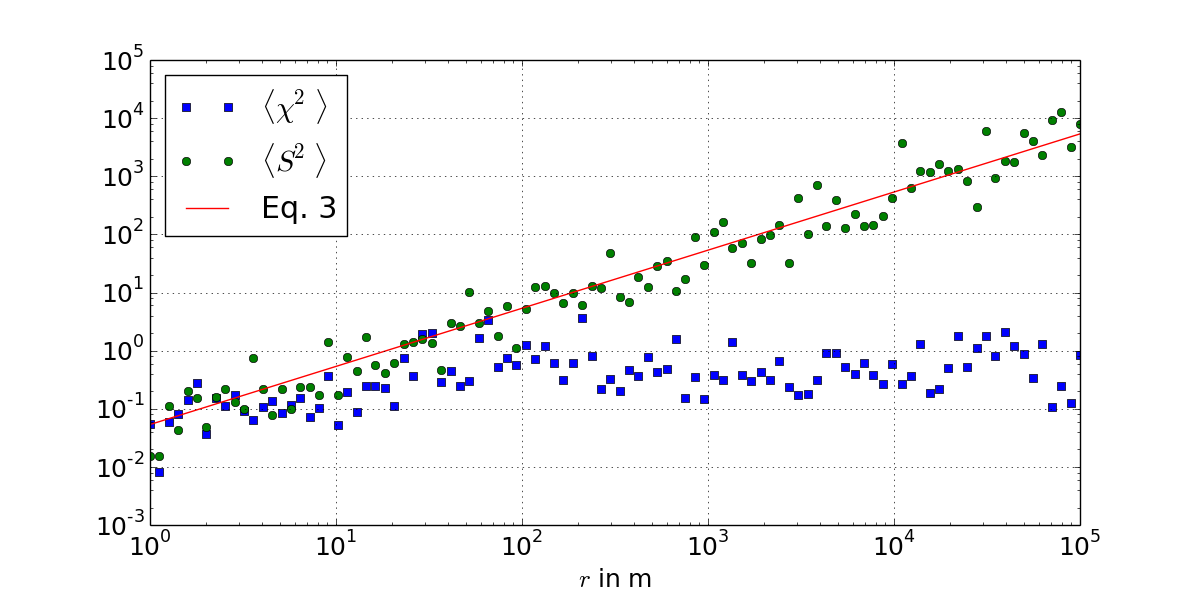
\includegraphics[width=75mm]{../figures/function_of_distance_with_saturation}}}


Finally, the modulation signal was applied to a tone of the same frequency as the modulation signal was calculated for. The resulting signal is shown in figure \ref{fig:levels}.
\Figure{fig:levels}{Sound pressure level $L_p$ of a signal modulated by the modulation signal shown in figure \ref{fig:modulation_signal}.
The input signal is a sine wave of 200 Hz. Time-weighting 'F' was used. The standard deviation of this modulated signal is 7 dB.}
       {60}{ \put(3,3)  {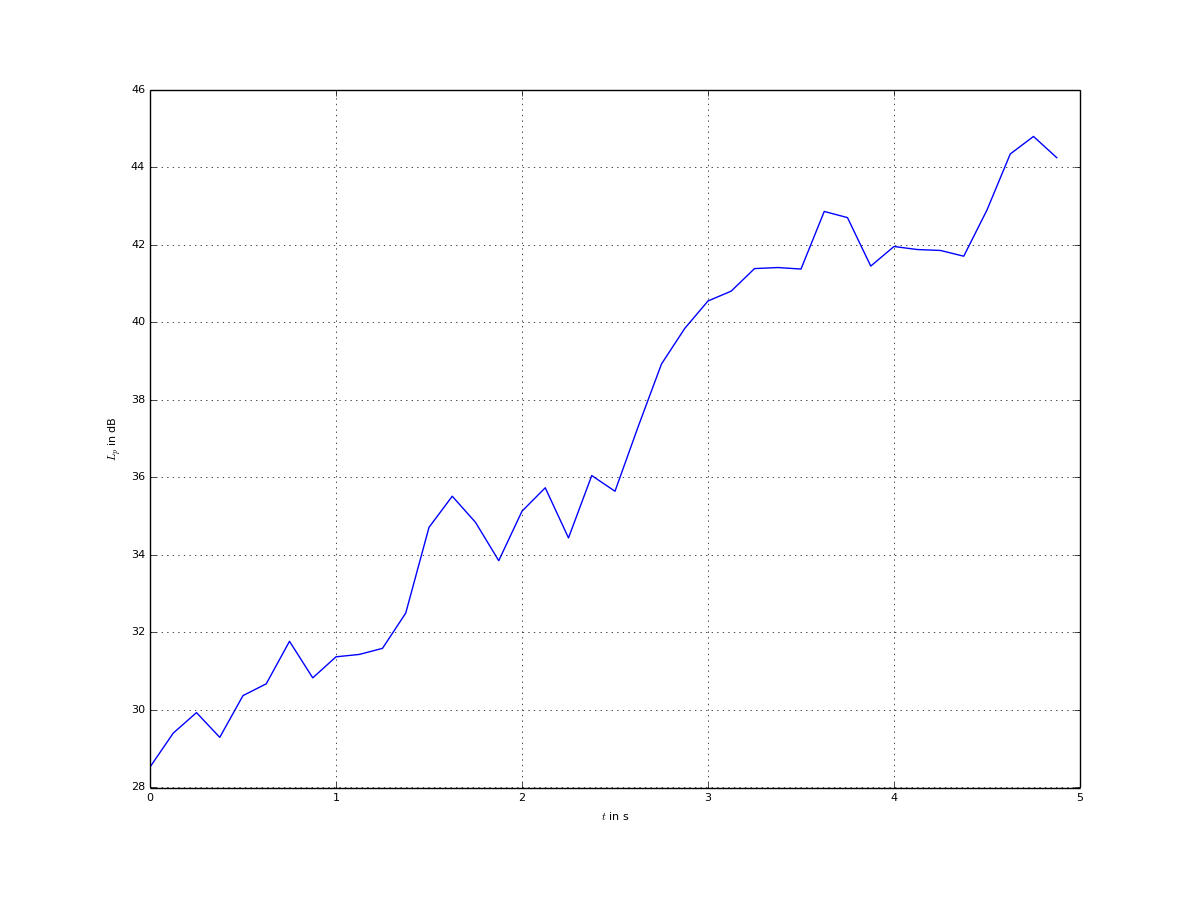
\includegraphics[width=75mm]{../figures/levels}}}
